\section{Results}
\label{section:results}

We have implemented the algorithm in Section \ref{section:algorithm}
in a tool called \texttt{CRTSolver} which is available at
\url{https://github.com/maheenmatin/CRTSolver} under the MIT license.
%
It uses two instances of cvc5, one to solve the modulo sub-problems
and a second to check the candidate results.  The following options
are available: Integer Mode and Bit-Vector Mode. 

Integer Mode attempts to
solve the modulo subproblem using the theory of Quantifier-Free Nonlinear
Integer Arithmetic, where the variables are of integer sort and integer
operations are used. 
Bit-Vector Mode uses the theory of Quantifier-Free
Bit-Vector Logic, where the variables are of bit-vector sort (with a fixed
bit-width calculated as a function of the current prime) and bit-vector
operations are used.
For the checking of candidate results, the theory of Quantifier-Free
Nonlinear Integer Arithmetic is used for both Integer Mode and Bit-Vector
Mode.

We have created a set of benchmarks that evaluate the performance of CRTSolver 
in both available modes on non-linear integer equations, in comparison with two
widely used and state-of-the-art SMT solvers, Z3 and cvc5.
The benchmarks are time and success rate, where time simply refers to the total runtime
for a given equation in milliseconds. We define a successful solving of a given
equation as termination with \texttt{SAT} or \texttt{UNSAT} - if a solver terminates
with \texttt{UNKNOWN} due to time constraints, memory constraints, or internal error,
then we define this as an unsuccessful solving.


\mmsays{Added Harvard in-text citation
and @inproceedings in .bib}

In Table \ref{table:results} we give a comparison with Z3 (de Moura and Bj{\o}rner, 2008) and 
cvc5 (Barbosa et al., 2022). 
The performance evaluation was conducted using a Juypter Notebook file on Visual Studio Code (version 1.100).
WSL2 (Ubuntu) was used on a Windows 11 Home (version 10.0.26100) PC with an Intel i5-11400 processor and 
16GB of RAM. The respective Python APIs for the latest versions of Z3 (version 4.14.1.0) and cvc5 
(version 1.2.1) at the time of testing were used.

All solvers had their available memory limited to 4GB and were given the same time-out value 
(the time limit for each \texttt{check-sat}) of 10 seconds. They were all given the same 30 test 
files, which were in the form of SMT2 files containing non-linear integer equations. Files were divided into 3 
groups: equations involving 1 variable, equations involving 2 variables and equations involving 3 variables. 
Each of these groups contained sub-groups of quadratic and cubic equations. There was a mixture of both 
satisfiable and unsatisfiable equations - however, there was a slight bias for the frequency of unsatisfiable 
cubic equations as these were found to be the most demanding equations, thus making them especially suitable 
for evaluating performance.

For each equation, we give the number of variables present, the degree, and whether or not the equation is 
satisfiable. CRTSolver's Integer Mode and Bit-Vector mode have been represented using the column headings 
\texttt{CRT-INT} and \texttt{CRT-BV} respectively. For each solver, the time taken for the equation is given. 
If the solver was successful in solving the given equation, we simply provide this in seconds. Where
the runtime is greater than or equal to 1 second it is represented with 3 decimal places, and if less 
than 1 second it is represented in scientific notation with 3 significant figures. 
However, the solver may be unsuccessful due to
a number of reasons, therefore terminating with \texttt{UNKNOWN}. In the case of exceeding the time-out value,
we denote this with \texttt{T/O} - note that in every such instance the runtime is equal to the 
time-out value of 10 seconds. Finally, in the case of integer overflow during solving, we denote this 
with \texttt{I/O} and provide the runtime before termination with integer overflow.
These results are also shown in a cactus plot in Figure \ref{figure:cactus-plot}.
All results were produced using v1.0.0 of CRTSolver.

\begin{table*}
  \caption{Performance Comparison between CRTSolver, Z3 and cvc5.}
  \label{table:results}
  \begin{tabular}{ccccccccc}
    \toprule
    Variables & Degree & SAT & CRT-INT & CRT-BV & Z3 & cvc5 \\
    \midrule
1 & 2 & UNSAT & T/O & $3.17 \times 10^{-02}$ & $4.41 \times 10^{-03}$ & $8.43 \times 10^{-03}$ \\
1 & 2 & SAT & $2.20 \times 10^{-01}$ & $1.25 \times 10^{-02}$ & $7.64 \times 10^{-03}$ & $4.85 \times 10^{-03}$ \\
1 & 2 & SAT & $4.12 \times 10^{-01}$ & $5.02 \times 10^{-03}$ & $3.97 \times 10^{-03}$ & $2.26 \times 10^{-03}$ \\
1 & 2 & UNSAT & T/O & $5.77 \times 10^{-03}$ & $3.63 \times 10^{-03}$ & $5.20 \times 10^{-03}$ \\
1 & 2 & SAT & $3.10 \times 10^{-01}$ & $6.98 \times 10^{-03}$ & $3.76 \times 10^{-03}$ & $2.61 \times 10^{-03}$ \\
1 & 2 & UNSAT & T/O & $1.80 \times 10^{-02}$ & $3.35 \times 10^{-03}$ & $4.11 \times 10^{-03}$ \\
1 & 2 & UNSAT & T/O & $4.56 \times 10^{-02}$ & $4.12 \times 10^{-03}$ & $2.32 \times 10^{-03}$ \\
1 & 3 & UNSAT & T/O & $1.74 \times 10^{-01}$ & $3.30 \times 10^{-03}$ & T/O \\
1 & 3 & SAT & $8.41 \times 10^{-03}$ & $2.17 \times 10^{-02}$ & $3.93 \times 10^{-03}$ & $7.00 \times 10^{-03}$ \\
1 & 3 & SAT & $8.43 \times 10^{-03}$ & $4.89 \times 10^{-03}$ & $3.76 \times 10^{-03}$ & $7.78 \times 10^{-03}$ \\
1 & 3 & SAT & $4.29 \times 10^{-01}$ & $2.69 \times 10^{-02}$ & $3.54 \times 10^{-03}$ & $2.75 \times 10^{-01}$ \\
1 & 3 & UNSAT & T/O & $1.80 \times 10^{-02}$ & $1.61 \times 10^{-02}$ & T/O \\
1 & 3 & UNSAT & T/O & $7.00 \times 10^{-03}$ & $1.21 \times 10^{-02}$ & T/O \\
2 & 2 & UNSAT & T/O & I/O ($7.10 \times 10^{-01}$) & $4.65 \times 10^{-03}$ & $1.89 \times 10^{-01}$ \\
2 & 2 & SAT & $3.34 \times 10^{-01}$ & $5.38 \times 10^{-02}$ & $3.41 \times 10^{-03}$ & $5.87 \times 10^{-02}$ \\
2 & 2 & SAT & $2.05 \times 10^{-01}$ & $9.71 \times 10^{-03}$ & $7.88 \times 10^{-03}$ & $1.612$ \\
2 & 2 & UNSAT & T/O & I/O ($5.69 \times 10^{-01}$) & $1.90 \times 10^{-03}$ & $3.02 \times 10^{-01}$ \\
2 & 3 & SAT & $2.80 \times 10^{-01}$ & $3.09 \times 10^{-02}$ & $3.30 \times 10^{-03}$ & $2.12 \times 10^{-01}$ \\
2 & 3 & UNSAT & T/O & I/O ($2.98 \times 10^{-01}$) & T/O & T/O \\
2 & 3 & UNSAT & T/O & I/O ($4.29 \times 10^{-01}$) & T/O & T/O \\
2 & 3 & SAT & $1.14 \times 10^{-02}$ & $1.45 \times 10^{-02}$ & $2.34 \times 10^{-03}$ & $4.37 \times 10^{-03}$ \\
2 & 3 & UNSAT & T/O & I/O ($3.57 \times 10^{-01}$) & T/O & $1.34 \times 10^{-01}$ \\
2 & 3 & UNSAT & $8.04 \times 10^{-03}$ & $5.24 \times 10^{-03}$ & $1.82 \times 10^{-03}$ & $8.02 \times 10^{-03}$ \\
3 & 2 & SAT & $1.75 \times 10^{-01}$ & $6.58 \times 10^{-02}$ & $3.71 \times 10^{-03}$ & $4.14 \times 10^{-01}$ \\
3 & 2 & SAT & $3.75 \times 10^{-02}$ & $3.85 \times 10^{-02}$ & $3.26 \times 10^{-03}$ & $9.83 \times 10^{-03}$ \\
3 & 3 & UNSAT & T/O & I/O ($1.767$) & T/O & T/O \\
3 & 3 & SAT & $4.58 \times 10^{-02}$ & $5.75 \times 10^{-02}$ & $3.24 \times 10^{-03}$ & $8.96 \times 10^{-03}$ \\
3 & 3 & SAT & $1.54 \times 10^{-01}$ & $6.79 \times 10^{-02}$ & $3.99 \times 10^{-03}$ & $1.368$ \\
3 & 3 & UNSAT & T/O & I/O ($1.252$) & T/O & T/O \\
3 & 3 & UNSAT & T/O & I/O ($1.798$) & T/O & T/O \\
  \bottomrule
\end{tabular}
\end{table*}

\mmsays{Please check the following equations for satisfiability (I think they are UNSAT):
$53(x-29)^3 + 61(y-16)^3 + 83(z+12)^3 = 51$
$13(x-1)^3 + 3(y-11)^3 + 17(z+19)^3 = -101$
$(x+23)^3 + (y-51)^3 + (z+39)^3 = -43$
}


\begin{figure*}
    \vspace{4em}
    \centering
    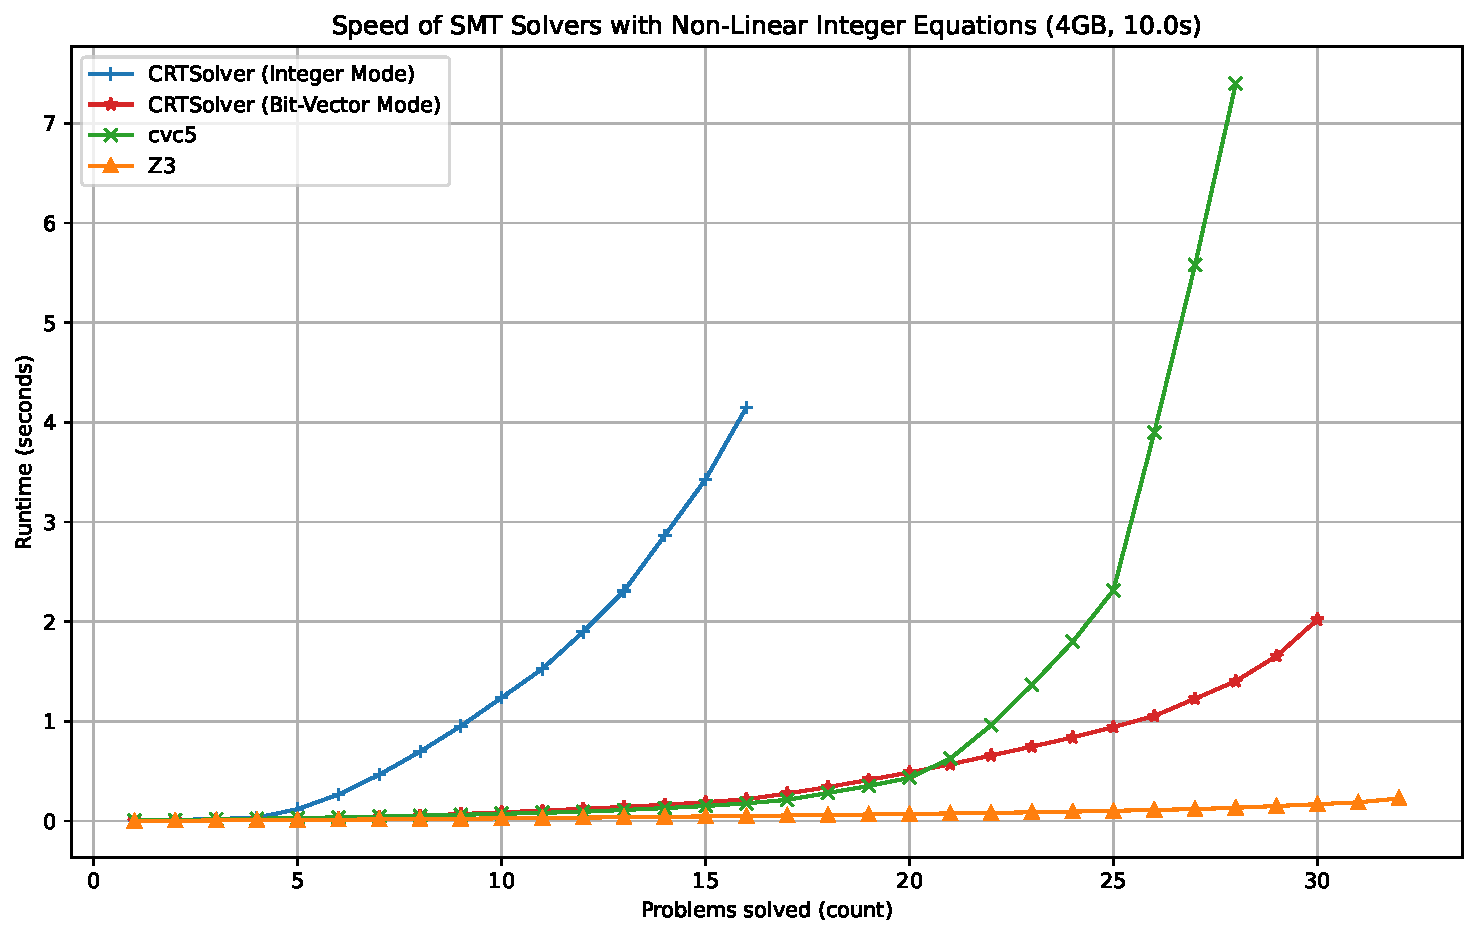
\includegraphics[width=1.0\linewidth]{cactus.pdf}
  \caption{A cactus plot of the results.}
  \label{figure:cactus-plot}
\end{figure*}

These results suggest that there using CRTSolver realistic potential in using CRTSolver in Bit-Vector Mode
as a solver that offers equal or better performance than existing solvers for non-linear
integer equations. However, the Integer Mode of CRTSolver can be safely concluded as having no real potential.
